
%
% Background Chapter
% Jason Brownlee
%

% What I want the reader to know about before getting stuck into my research

% Guideline: Audience is the Lay-reader

% Assessment: 
% Has the author examined a suitable range of recent periodicals and determined key researchers and journals?  Has the author provided and evaluated a range of different, professional views on the subject at hand?  Has the author explained how each cited reference contributed to the directions of the research?  Have references been correctly cited where used?


%
% Background
%
\chapter{Background}
\label{chap:background}

%
% Overview
% Provides an overview of the chapter and its structure, and a description of what is intended to be achieved by providing this documentation. A description of why and how this chapter follows on from the previous chapter
%
\section{Chapter Overview}
\label{sec:background:overview}
% general
This chapter provides background information and reviews the base motivations for the work. 
% position
Section~\ref{sec:aiandci} generally positions the work within the sub fields of Biologically Inspired Computation and Computational Intelligence under the broader field of Artificial Intelligence. Section~\ref{sec:background:isandais} clarifies this further by outlining the specific field of Artificial Immune Systems. 
% cs
Section~\ref{sec:background:threeschools} reviews the core paradigms in the field, highlighting the cellular focus that inspires the computational approaches, and the general fundamental role the adaptive clonal selection strategy has across the field.
% dais
Section~\ref{sec:background:distributedais} motivates the specific research hypothesis of this work in the development of distributed Artificial Immune Systems, and how the this decentralised adaptive property is generally promoted in the field, although remains underdeveloped.
% biology
Section~\ref{sec:background:openproblems} reviews open problems in the field, highlighting the general impasses and lack of satisfying progress and advocating the specific approach taken in this work of turning back to the motivating metaphor toward developing more sophisticated approaches.
% methodology
Finally, a systematic methodology is pieced together in Section\ref{sec:background:methodology} from best practices with regard to (1) biologically inspired algorithm development, (2) experimental investigation, and (3) the economy of modelling and integration of findings.
% next chapter
This chapter sets the scene for the following chapter that outlines the specific elaborations and distributed realisations of clonal selection investigated throughout the remainder of the dissertation.


%
% AI and CI
% Omitted the advantages and disadvantages of the field (BIC)
%
\section{Artificial and Computational Intelligence}
\label{sec:aiandci}

%
% Artificial Intelligence
%
\subsection{Artificial Intelligence}
The general field of study is the multi-disciplinary field of Artificial Intelligence (AI). Russell and Norvig provide a perspective that defines Artificial Intelligence in four categories: (1) systems that think like humans, (2) systems that act like humans, (3) systems that think rationally, (4) systems that act rationally \cite{Russell1995}. In the definition, acting like a human suggests that a system can do some specific things humans can do, this includes fields such as the Turing test, natural language processing, automated reasoning, knowledge representation, machine learning, computer vision, and robotics. Thinking like a human suggests systems that model the cognitive information processing properties of humans, for example a general problem solver and systems that build internal models of their world. Thinking rationally suggests laws of rationalism and structured thought, such as syllogisms and formal logic. Finally, acting rationally suggests systems that do rational things such as expected utility maximisation and rational agents. Luger and Stubblefield suggest that AI is a sub-field of computer science concerned with the automation of intelligence, and like other sub-fields of computer science has both theoretical (\emph{how and why do the systems work?}) and application (\emph{where and when can the systems be used?}) concerns \cite{Luger1997}. They suggest a strong empirical focus to research, such that although there may be a strong desire for mathematical analysis, the systems themselves defy analysis due to their complexity. The machines and software themselves are not black boxes, rather analysis proceeds by observing the systems interactions with their environment, followed by an internal assessment of the system to relate their structure back to their behaviour. 

Artificial Intelligence is therefore concerned with investigating mechanisms that underlie intelligence and intelligence behaviour. The traditional approach toward designing and investigating AI (the so-called `good old fashioned' AI) has been to employ a symbolic basis for these mechanisms. A newer approach historically referred to as \emph{messy artificial intelligence} or or \emph{soft computing} does not use a symbolic basis, instead patterning these mechanisms after biological or natural processes. This represents a modern paradigm shift in interest from symbolic knowledge representations, to inference strategies for adaptation and learning, and has been referred to as \emph{neat} versus \emph{scruffy} approaches to AI. The neat philosophy is concerned with formal symbolic models of intelligence that can explain \emph{why} they work, whereas the scruffy philosophy is concerned with intelligent strategies that explain \emph{how} they work \cite{Sloman1990}.


%
% Computational Intelligence
%
\subsection{Computational Intelligence}
% CI
A modern name for the sub-field of AI concerned with sub-symbolic (messy, scruffy, soft) mechanisms is \emph{Computational Intelligence}. This name provides a banner which groups four principle approaches: Fuzzy Intelligence, Connectionist Intelligence, Evolutionary Intelligence, and Swarm Intelligence \cite{Engelbrecht2002, Pedrycz1997}. 
% metaheuristcs
A second popular and general name for the \emph{strategy}-\emph{outcome} perspective of scruffy AI is \emph{Metaheuristics}, which evolved from the neater field of heuristics methods applied in Operations Research. A metaheuristic is defined as a general algorithmic framework which can be applied to different optimisation problems with relative few modifications to make them adapted to a specific problem \cite{Blum2003}. 
% machine learning
Another important perspective is that provided by the field of \emph{Machine Learning} that focuses on the learning properties of Artificial Intelligence. The term is commonly used to describe inductive model building techniques (that generalise from specific observations) that are applied to `learn' relationships in data sets (the application of which is referred to as Data Mining \cite{Witten2000}), with or without supervision (corrective behaviour) \cite{Michalski1983}. 
% list
The following provides a summary of the four primary areas of study in Computational Intelligence:

\paragraph{Evolutionary Computation} A paradigm that is concerned with the investigation of systems inspired by the neo-Darwinian theory of evolution by means of natural selection. Popular evolutionary algorithms include the Genetic Algorithm, Evolution Strategy, Genetic and Evolutionary Programming, and Differential Evolution. The evolutionary process is considered an adaptive strategy and is typically applied to search and optimisation domains.
\paragraph{Swarm Intelligence} A paradigm that considers collective intelligence emerges through the interaction and cooperation of large numbers of lesser intelligent agents. The paradigm consists of two dominant sub-fields (1) \emph{Ant Colony Optimisation} that investigates probabilistic algorithms inspired by the stigmergy and foraging behaviour of ants, and (2) \emph{Particle Swarm Optimisation} that investigates probabilistic algorithms inspired by the flocking and foraging behaviour of birds and fish. Like evolutionary computation, swarm intelligences are considered adaptive strategies and are typically applied to search and optimisation domains.
\paragraph{Connectionist Intelligence} An approach that is concerned with the investigation of architectures and learning strategies inspired by the  modelling of neurons in the brain called \emph{Artificial Neural Networks}. Learning strategies are typically divided into supervised and unsupervised which manage environmental feedback in different ways. Neural network learning processes are considered adaptive learning and are typically applied to pattern recognition domains.
\paragraph{Fuzzy Intelligence} An approach that is concerned with the investigation of fuzzy logic which is a form of logic that is not constrained to true and false, but rather functions which define degree's of truth. Fuzzy logic is reasoning strategy and is typically applied to expert system and control system domains.

%
% Natural Computation
%
\subsection{Natural Computation}
An important perspective on scruffy Artificial Intelligence is the motivation and inspiration for the core information processing strategy of a given technique. Computers can only do what they are instructed, therefore a consideration of Computational Intelligence is to distil information principles and strategies from other fields of study, such as biology. The study of biologically motivated Computational Intelligence may be called \emph{Biologically Inspired Computing} \cite{Castro2005}, and is one of three related fields of \emph{Natural Computing} \cite{Forbes2000, Forbes2004, Paton1994}. Natural Computing is an interdisciplinary field concerned with the relationship of computation and biology, which in addition to Biologically Inspired Computing also comprises of \emph{Computationally Motivated Biology} and \emph{Computing with Biology} \cite{Paun2005, Marrow2000, Aaronson2005}. Therefore, the field of Artificial Intelligence, specifically the scruffy variety of Computational Intelligence motivates this work from the perspective of an intelligent problem-solving strategy in computer science, whereas the field of Natural Computing, specifically the Biological Inspired Computation variety motivates the actual principles and information processing capabilities of the strategy.

\paragraph{Biologically Inspired Computation} (\emph{Computation inspired by biological metaphor}) The intent is to devise mathematical or engineering tools to address problem domains. Biologically Inspired Computation fits into this category, as do other non-computational areas of problem solving not discussed. At its simplest, its using solutions (a procedure for finding solutions is considered a solution) found in the biological environment.
\paragraph{Computationally Motivated Biology} (\emph{Biology with digital computers}) The intent of this area is to use information sciences and simulation to model biological systems in digital computers with the aim to replicate and better understand behaviours in biological systems. The field facilitates the ability to better understand life-as-it-is and investigate life-as-it-could-be. Typically, work in this sub-field is not concerned with the construction of mathematical and engineering tools, rather it is focused on simulating natural phenomena. Common examples include Artificial Life, Fractal Geometry (L-systems, Iterative Function Systems, Particle Systems, Brownian motion), and Cellular Automata.
\paragraph{Computing with Biology} The investigation of substrates other than silicon in which to implement computation. Common examples include molecular or DNA Computing and Quantum Computing.

%
% Natural and Artificial Immune Systems 
%
\section{Natural and Artificial Immune Systems}
\label{sec:background:isandais}
This section reviews the biological immune system which motivates the biologically inspired field of Artificial Immune Systems. The varied approaches in this field have lead to some debate as to how it relates to sibling Computational Intelligence sub-fields, comprising features from Evolutionary Computation, Swarm Intelligence, and Connectionist Intelligence. These relationships are further considered in Section~\ref{sec:cs:related}.

%
% Mammalian Immunology
%
\subsection{Overview of the Immune System}
\label{sec:immunology}
This review of the immune system with a focus on the general problem to which the biological system is attributed to addressing, which is to protect the host organism from the threats posed to it from pathogens and toxic substances. Pathogens encompass a range of micro-organisms such as bacteria, virus, parasites and pollen. This review provides sufficient immunology such that a computer scientist may grasp the core architecture, processes and general problem of addressed by the immune system. The focus is the vertebrate immune system, specifically that of mammals given that disproportionally more information is known about the system. For more general information, the reader is directed to two addition reviews of immunology by and for Computer Scientists, de~Castro and Timmis \cite{Castro2002b} (Chapter 2), and Hofmeyr \cite{Hofmeyr2001}.

The traditional perspective regarding the role of the immune system is divided into two primary tasks: the \emph{detection} and \emph{elimination} of pathogen\footnote{More recent perspectives on the role of the system include a maintenance system \cite{Cohen2001a}, and a cognitive system \cite{Varela1994}.}. This behaviour is typically referred to as the differentiation of self (molecules and cells that belong to the host organisms) from potentially harmful non-self. The architecture of the immune system is such that a series of defensive layers protect the host. The most basic of these layers provide \emph{physical barriers} to prevent pathogen from entering the host such as skin, and mucous membranes that trap and filter out pathogen. The next level is physiological that provides inhospitable conditions for pathogen at entry points to host such as high pH acidity in the digestive tract and varied temperature to inhibit growth of micro-organisms. Once a pathogen makes it inside the host, it must contend with the \emph{innate} and \emph{acquired} immune system. These interrelated immunological sub-systems are comprised of many types of cells  and molecules produced by specialised organs and processes to address the self-nonself problem at the lowest level using chemical bonding, where the surfaces of cells and molecules interact with the surfaces of pathogen.

%
% Innate Immunity
%
\subsubsection{Innate Immunity}
The innate immune system is named such because the host organism is born with a set of fast acting detection and elimination mechanisms that do not change over the hosts lifetime. In this regard, the mechanisms are reflexive providing a \emph{first line of defence} against pathogen. Innate mechanisms are the most primitive found in all classes of plant and animal life improving in a species over evolutionary time. 
% more
The complement system refers to a mechanism where associated molecules bind to and coat specific types of bacteria. The activation of this mechanism (a complement cascade) can lead to a rupturing of the bacteria called \emph{lysis}, or detection and subsequent killing of the bacteria by macrophage cells called \emph{opsonisation}. The process is fast acting, typically occurring within a the first few hours of an infection. Macrophages are scavenger cells responsible for cleaning up cellular debris, some bacteria, and micro-organisms that have been identified by the complement system. These cells engulf material and neutralise it using a digestive process. When a virus infects a cell, the cell may release chemicals called cytokines that provide an indication to other cells of the infection. \emph{Natural Killer} (NK) cells are a specialised class of immune cell responsible for identifying virally infected cells via their chemical signals and releasing chemicals that trigger apoptosis (programmed cell death) of these cells. These NK cells are also responsible for identifying and eliminating tumour cells. 

%
% Adaptive Immunity
%
\subsubsection{Adaptive Immunity}
The adaptive immune system, also referred to as the acquired immune system, is named such because it is responsible for specialising a defence for the host organism based on the \emph{specific} pathogen to which it is exposed. Unlike the innate immune system, the acquired immune system is present only in vertebrates (animals with a spinal column). The system retains a \emph{memory} of exposures which it has encountered. This memory is \emph{recalled} on reinfection exhibiting a \emph{learned} pathogen identification. This learning process may be divided into two types of response. The first or \emph{primary response} occurs when the system encounters a novel pathogen. The system is slow to respond, potentially taking a number of weeks to clear the infection. On re-encountering the same pathogen again, the system exhibits a \emph{secondary response}, applying what was learned in the primary response and clearing up the infection rapidly. The \emph{memory} the system acquires in the primary response is typically long lasting, providing pathogenic immunity for the lifetime of the host, two common examples of which are the chickenpox and measles. White blood cells called lymphocytes (or leukocytes) are the most important cell in the acquired immune system. Lymphocytes are involved in both the identification and elimination of pathogen, and recirculate within the host organisms body in the blood and lymph (the fluid that permeates tissue). The behaviour of the adaptive immune system may be described with regard to two general sub-systems: \emph{Humoral Immunity} for addressing free-floating pathogen (for example in blood), and \emph{Cellular Immunity} for addressing virally infected cells.

\paragraph{Humoral Immunity} B-lymphocyte cells are a specialised class of white blood cell that are created in the bone marrow and are predominantly responsible for the secretion of antibodies. These are protein molecules that bind to parts or specialised features of pathogen called pathogenic determinants. B-cells are activated by identifying pathogen via their surface bound receptors which provide a complementary shape for pathogen surface features, fitting like a lock and a key. Once activated a B-cell will produce vast quantities of antibody which enter the blood stream and recirculate around the host organism to clear up the infection.

\paragraph{Cellular Immunity} T-lymphocyte cells are another class of white blood cell that are matured in the thymus (an immune organ located in the chest). T-cells perform specific roles both mediating the activation of B-cells (Helper T-cells) and in the identification and neutralisation of virally infected cells (Killer T-cells). In this latter role, T-cells identify processed (chopped up) pieces of pathogen on the surfaces of infected cells called histocompatibility complex (commonly referred to by its abbreviation: MHC). Cells responsible for processing pathogen and presenting MHC are appropriately called antigen-presenting cells, examples of which include some B-cells, macrophages and dendritic cells.

%
% Artificial Immune Systems (AIS)
%
\subsection{Artificial Immune Systems}
\label{sec:ais}

%
% History
%
\subsubsection{History}
Artificial Immune Systems (AIS) is a sub-field Computational Intelligence motivated by immunology (primarily mammalian immunology) that emerged in the early 1990's (for example \cite{Bersini1990, Ishida1990}), based on the proposal in the late 1980's to apply  theoretical immunological models to machine learning and automated problem solving (such as \cite{Hoffmann1986, Farmer1986a}). The early works in the field were inspired by exotic theoretical models (immune network theory) and were applied to machine learning, control and optimisation problems. The approaches were reminiscent of paradigms such as Artificial Neural Networks, Genetic Algorithms, Reinforcement Learning, and Learning Classifier Systems. The most formative works in giving the field an identity were those that proposed the immune system as an analogy for information protection systems in the field of computer security. The classical examples include Forrest, et~al.'s Computer Immunity \cite{Forrest1994a, Forrest1997a} and Kephart's Immune Anti-Virus \cite{Kephart1994, Kephart1995}. These works were formative for the field because they provided an intuitive application domain that captivated a broader audience and assisted in differentiating the work as an independent sub-field.

%
% Motivation
%
\subsubsection{Motivation}
The motivation for the field of AIS is the immune system, specifically the architecture, mechanisms, principles, and theories used to explain observed immunological function. The authors de~Castro and Timmis defend the immune system as an inspiration for computational intelligence by providing a comprehensive listing of abstracted information processing principles \cite{Castro2002b} (pages 55-56). This listing contains nineteen desirable computational attributes, the following of which specifically motivate this research:

\begin{itemize}
	\item \emph{Uniqueness}: Each individual with an immune system has distinct and different capabilities and vulnerabilities.
	\item \emph{Disposability}: There is no single cell or molecule that is essential to the functioning of the immune system.
	\item \emph{Autonomy}: There is no central or coordinating organ controlling the immune system
	\item \emph{Distributivity}: The immune cells, molecules, and organs are distributed all over the body and are not subject to centralised control.
	\item \emph{Fault Tolerance}: The complementary roles performed by several immune components allow the re-allocation of resources in the event of failure.
	\item \emph{Self-Organisation}: There is no specific information as to how to respond to a given pathogen, the system responds locally providing a global effect of defence.
\end{itemize}

Forrest and Hofmeyr take a similar approach in considering and abstracting the information processing principles of the immune system \cite{Forrest2001}. In their work, the authors focus on three specific information-processing principles, although they highlight a number of general design principles that have much overlap with the de~Castro-Timmis listing. Perhaps the more important features that strongly entrench the field of Computational Intelligence are \emph{Immune Learning} (acquired information through interaction with the environment) and \emph{Immune Memory} (persistence and ongoing application of acquired information for short and long durations), both of which fit into a broad notion of intelligence. Using this general description, the mammalian acquired immune system may be considered rudimentary intelligent. 

%
% Definitions
%
\subsubsection{Definitions}
Although the motivations of the field are easy to relate, it is important to clarify those motivations that do not contribute to the specific field. This section focuses on some standard definitions of what is and is not an Artificial Immune System. The authors de~Castro and Von Zuben \cite{Castro2000a} define an AIS as ``\emph{a computational system based upon metaphors of the biological immune system}''. They continue by defining \emph{Immune Engineering} as the application of an AIS in ``\emph{a meta-synthesis process that uses the information contained in the problem itself to define the solution tool to a given problem, and then apply it to obtain the problem solution}''. The distinction is that Immune Engineering is the engineering process, differentiated from conventional engineering process via its biological (immunological) motivation. Immune Engineering was later formalised into a framework by de~Castro and Timmis as a set of three principles of what an Artificial Immune System should contain \cite{Castro2002a}, as follows: (1) A representation for the components of the system, (2) A set of mechanisms to evaluate the interaction of individuals with the environment and each other, and (3) Procedures of adaptation that govern the dynamics of the system.

A further, more concise definition of AIS is provided in the same work as ``\emph{adaptive systems, inspired by theoretical immunology and observed immunological functions, principles and models, which are applied to problem solving}''. This definition clearly highlights the role of theoretical immunology and immunological observations as an inspiration and not the pursuit of research in AIS, and is the definition adopted in this dissertation. In addition to the clarification it provides, the authors propose that a system to be referred to as an AIS must incorporate a minimum level of immunology, such as an immune component (for example cell, molecule, and organ), it has to be designed by incorporating ideas from theoretical and/or experimental immunology, and it has to be directed toward problem solving. They stipulate that attributing immunological terminology is insufficient to call a system an artificial immune system.

Another perspective of AIS is provided by one of the pioneers in the field Ishida who defines an Immunity-Based System (IMBS) as a ``\emph{self-maintenance systems learned from and inspired by the immune system}''  \cite{Ishida2004}. His IMBS is described as (1) a \emph{self-maintenance system} with monitoring of self and nonself, (2) a \emph{distributed system} with autonomous components capable of mutual evaluation, and (3) an \emph{adaptive system} with diversity and selection. The three properties of Ishida's AIS complement the de~Castro-Timmis definition by highlighting core information processing characteristics as a baseline when abstracting from the biological system that may be distilled to (\emph{autonomy}, \emph{distributed}, \emph{adaptive}). 


%
% Three Schools of Artificial Immune Systems
%
\section{Three Schools of AIS}
\label{sec:background:threeschools}
This section provides a summary of the field of Artificial Immune Systems. The review presents a taxonomy that covers the three core paradigms employed that collectively cover the majority of the work in the field: \emph{Clonal Selection}, \emph{Negative Selection}, and \emph{Immune Network}. Each paradigm is presented from the perspective of immunological theory of immune cell interactions, the abstracted information processing principles, and the algorithms and applications that have been proposed. 
% cs focus
As such, the review highlights the central role the adaptive clonal selection theory plays across the principles paradigms in the field.

%
% Clonal Selection Paradigm
%
\subsection{Clonal Selection Paradigm}
\label{subsec:background:clonalselection}
% theory
The clonal selection theory credited to Frank Macfarlane Burnet was proposed to account for the behaviour and capabilities of antibodies in the acquired immune system \cite{Burnet1957, Burnet1959}. Inspired by the principles of Darwinian natural selection theory of evolution, the theory proposes that antigens select-for lymphocytes (both B and T-cells). When a lymphocyte is selected and binds to an antigenic determinant, the cell proliferates making many thousands more copies and differentiates into different cell types (plasma and memory cells). Plasma cells have a short lifespan and produce vast quantities of antibody molecules, whereas memory cells live for an extended period in the host anticipating future recognition of the same determinant. The important feature of the theory is that when a cell is selected and proliferates, it is subjected to small copying errors (changes to the genome called somatic hypermutation) that change the shape of the expressed receptors and subsequent determinant recognition capabilities of both the antibodies bound to the lymphocytes cells surface, and the antibodies that plasma cells produce. 

% information processing
The theory is interesting from an information processing perspective. It suggests that starting with an initial repertoire of general immune cells, the system is able to change itself (the compositions and densities of cells and their receptors) in response to experience with the environment. Through a blind process of selection and accumulated variation on the large scale of many billions of cells, the acquired immune system is capable of acquiring the necessary information to protect the host organism from the specific pathogenic dangers of the environment. It also suggests that the system must anticipate (guess) at the pathogen to which it will be exposed, and requires exposure to pathogen that may harm the host before it can acquire the necessary information to provide a defence.

% quintessential algorithms
The information processing principles of the clonal selection theory describe a general learning strategy. The theory has inspired a suite of algorithms for optimisation, classification, and other rudimentary machine learning problem domains. In each algorithm, a population of adaptive information units (each representing a problem-solution or component thereof) is subjected to a competition processes for selection, which together with the resultant duplication and variation, ultimately improves the information units, and solves or approximately solves a problem. The seminal algorithm was proposed by de~Castro called the CLONal selection ALGorithm (CLONALG) \cite{Castro2000, Castro2002} and was applied to Function Optimisation, the Travelling Salesman Problem (a combinatorial optimisation problem) and Binary Character Pattern Recognition. Other algorithms include the B-cell Algorithm (BCA) \cite{Kelsey2003a, Kelsey2003}, and the Multi-objective Immune System Algorithm (MISA) \cite{Coello2002a, Cortes2003} for optimisation, and the Artificial Immune Recognition System (AIRS) by Watkins \cite{Watkins2002, Watkins2004a} for supervised classification. This paradigm is elaborated in Chapter \ref{chap:cs}.

%
% Negative Selection Paradigm
%
\subsection{Negative Selection Paradigm}
\label{subsec:background:negativeselection}
% Theory
An important consideration for Burnet in developing the clonal selection theory was the integration of the fact that such a powerfully destructive process as acquired immunity does not immediately turn against the host organism in the generation of self-antibodies (autoimmune response). This ability of the clonal response to maturate lymphocyte cells for pathogen and not self-tissues became known as \emph{self-nonself discrimination} \cite{Crist2000, Nossal1994}, and in conjunction with clonal selection forms paradigms by which the acquired immune systems is understood in the field of immunology. Clonal selection accounts for this observation by proposing both that (1) the initial repertoire of immune cells are prepared in such a way that none are autoimmune, and (2) that during the maturation process in the ongoing interaction with pathogen, that autoimmune clones are destroyed. Immune cells are continually being destroyed, therefore there is a constant stream of new immune cells that must be created and integrated into the repertoire. This theory was confirmed by the discovery of T-lymphocyte cells that are matured using both a positive and negative selection process in the thymus.

% information processing
Self-nonself discrimination primed with a negative selection process has interesting information processing properties. The theory suggests that the anticipatory guesses made in clonal selection are filtered by regions of infeasibility (protein conformations that bind to self-tissues). Further, the self-nonself immunological paradigm proposes the modelling of the unknown domain (encountered pathogen) by modelling the complement of what is known. This is unintuitive as the natural inclination is to categorise unknown information by what is different from what is known rather than guessing at the unknown information and filtering guesses by what is known. 

% algorithms
The information processing principles of the self-nonself discrimination via negative selection are that of a \emph{anomaly} and \emph{change} detection system that model the anticipation of variation from what is known. The seminal negative selection algorithm was proposed by Forrest, et~al. \cite{Forrest1994a} in which a population of detectors are prepared in the presence of known information, where those randomly generated detectors that match against known data are discarded. The population of pattern guesses in the unknown space then monitors the corpus of known information for changes. The algorithm was applied to the monitoring of files for changes (corruptions and infections by computer viruses), and later formalised as a change detection algorithm \cite{D'haeseleer1996a, D'haeseleer1996}. It was applied to monitoring changes in the execution behaviour of Unix processes \cite{Forrest1996, Hofmeyr1998}, and to monitor the changes in remote connections of a network computer (intrusion detection) \cite{Hofmeyr1999, Hofmeyr1999a}. The application of the algorithm has been predominantly to virus host intrusion detection and their abstracted problems of classification (two-class) and anomaly detection.
% validity
More recently, the validity of the application of negative selection algorithms in high-dimensional spaces has been questioned, specifically given the scalability of the approach in the face of the exponential increase in volume within the problem space \cite{Stibor2006}.

%
% Immune Network
%
\subsection{Immune Network Paradigm}
\label{subsec:background:immunenetwork}
% theory
A concern of the clonal selection theory is that it presumes that the repertoire of reactive cells remains idle when there are no pathogen to which to respond. Considering this problem, Niels Jerne proposed an Immune Network Theory (Idiotypic Networks) where immune cells are not at rest in the absence of pathogen, instead antibody and immune cells recognise and respond to each other \cite{Jerne1974a, Jerne1974, Jerne1984}. The theory proposes that antibody (both free floating and surface bound) possess idiotopes (surface features) to which the receptors of other antibody can bind. As a result of receptor interactions, the repertoire becomes dynamic, where receptors continually both inhibit and excite each other in complex regulatory networks (chains of receptors). The network theory suggests that the clonal selection process may be triggered by the idiotopes of other immune cells and molecules in addition to the surface characteristics of pathogen, and that the maturation process applies both to the receptors themselves the idiotopes which they expose. 

% information processing
The immune network theory has interesting resource maintenance and signalling information processing properties. The clonal selection and negative selection paradigms integrate the accumulative and filtered learning of the acquired immune system, whereas the immune network theory proposes an additional order of complexity between the cells and molecules under selection. In addition to cells that interact directly with pathogen, there are cells that interact with those reactive cells and with pathogen indirectly, in successive layers such that networks of activity for higher-order structures such as internal images of pathogen (promotion), and regulatory networks (so-called anti-idiotopes and anti-anti-idiotopes).

% quintessential algorithms
Early works, such as Farmer, et~al. \cite{Farmer1986a} suggested at the exploitation of the information processing properties of network theory for machine learning. A seminal network theory based algorithm was proposed by Timmis, et~al. called the Artificial Immune Network (AIN) \cite{Timmis2000a}  (later extended and renamed the Resource Limited Artificial Immune System \cite{Timmis2001, Timmis2000} and Artificial Immune Network \cite{Knight2001a}). The algorithm maintains a population of adaptive units that operate under a clonal selection process. Units are connected to each other based on distance measures in the information space (for example Euclidean distance if the units are real-valued vectors), such that adaptive units that are \emph{close} in the information space suppress the activation of each other. Therefore, the more \emph{connections} a given unit has with other nodes influences the units potential for being selected and cloned under clonal selection. Timmis' system was applied to feature extraction and data clustering. Another seminal network based algorithm was proposed by de~Castro and Von Zuben called Artificial Immune Network (aiNet) which extended the principles of AIN and CLONALG and was applied to clustering  \cite{Castro2000c, Castro2001a}. The aiNet algorithm was further extended to optimisation domains and renamed opt-aiNet \cite{Castro2002c}.

%
% Summary
%
\subsection{Summary}
\label{subsec:background:schools:summary}
% cs is important
The clonal selection, negative selection, and immune network paradigms represent the majority of the influences for the information processing properties from immunology exploited in the field of artificial immune systems. 
% other things
The proposed taxonomy is not complete, for example an additional influence that is not discussed is the Danger Theory of Polly Matzinger \cite{Matzinger1994, Matzinger2002} which proposes that the acquired immune system responds to signals of damage, which opposes the fundamental self-nonself paradigm. 
% cs is central
This coarse taxonomy of the field of Artificial Immune Systems clearly highlights the central role clonal selection to both the cognitive properties assigned to the immune system (learning and memory), and the three principle paradigms that underlie the field. This centrality and even reliance on clonal selection suggests that developments and improvements to the understanding of the paradigm will have follow-on effects to the other cell-based paradigms in the field. 


%
% Distributed Artificial Immune Systems
%
\section{Distributed Artificial Immune Systems}
\label{sec:background:distributedais}
One of the often cited propositions of using the immune system as an inspiration for computational systems is that it affords decentralised and distributed information processing. This section reviews this promise of the field of Artificial Immune Systems, and reviews systems and algorithms that have made progress toward this end. 

%
% Culture/Promise of Autonomy and Decentralised
% Promise of Distributed Information Processing
% (that does not follow through as far as I see)
%
\subsection{Promise of Distributed Information Processing}
\label{subsec:background:distributedais:promise}
The terms \emph{autonomous}, \emph{decentralised}, and \emph{distributed} are used with abandon in the field of Artificial Immune Systems to both describe information processing abstractions of the immune system and the desired characteristics of inspired systems. For example, the motivations and definitions for the in Section~\ref{sec:ais} both feature the distributed aspects of the immune system. Watkins, et~al. described the ``\emph{inherent distributedness}'' of the biological immune system, and the ``\emph{almost embarrassingly parallel nature}'' of the clonal selection algorithm \cite{Watkins2003}. Watkins and Timmis further pushed this perspective and commented that ``\emph{Among the oft-cited reasons for exploring the mammalian immune system as a source of inspiration for computational problem solving include the observations that the immune system is inherently parallel and distributed}'' \cite{Watkins2004}. Therefore, it is not unreasonable to consider that a promise of the field of Artificial Immune Systems is a source of distributed information processing paradigms, systems, and/or algorithms, imbued with notions of autonomy, decentralisation, parallelism, concurrency.

In this work, the terms are used with explicit meaning. \emph{Autonomy} refers to the self-governance of discrete facets of the system such as the molecules and cells and to the processes in which they are engaged for example the identification and neutralisation of pathogen. \emph{Decentralised} refers to the lack of centralised control, specifically the localisation of the self-governance such as at the spatial and temporal characteristics of a pathogenic encounter. Finally, \emph{distributed} is used in the systems sense of the integration and coordination of the localised self-governance of resources towards a holistic end, such as homoeostasis and general organism defence from infection. The definitions used align with the pursuit of Computational Intelligence systems that exploit the distributed information processing with multiple interacting and intelligent agents referred to as Distributed Artificial Intelligence and Multi-Agent Systems \cite{Weiss1999}. From Weiss' definition, the \emph{autonomy}, \emph{emergent cooperation} and \emph{intelligence} are preserved although the constraints of \emph{rationality}, \emph{local determinism}, and goal or \emph{task-directed behaviour} are relaxed in favour of the biologically inspired bottom-up and stochastic mechanisms of Computational Intelligence. Therefore, a distinction is made between centralised, distributed, and distributable, where a system may be designed or re-engineered to be \emph{distributed} although the benefits of such a process are not limited to concurrent, parallel, or distributed implementation in the computer hardware sense. 

%
% Review of Distributed Artificial Immune Systems
% Immune Inspired Distributed Algorithms and Systems
% (Case studies, examples, effort towards the distributed end)
%
\subsection{Algorithms, Systems, and Applications}
\label{subsec:distrb:review}
This section reviews the efforts towards the realisation of distributed Artificial Immune Systems. Considered in this review are the seminal works and main efforts toward such realisation which are categorised as (1) distributed negative selection approaches for computer security, (2) efforts toward autonomous and decentralised control systems and robotics, (3) network systems and application domains, (4) parallel extensions of existent algorithms, and (5) miscellaneous works.

%
% Detectors and Negative Selection
%
\subsubsection{Distributed Detectors for Computer Security}
\label{subsubsec:distrb:review:security}
% Distributed detector system
In their proposal of a distributed detection system based on the negative selection algorithm Forrest, et~al. comment on the characteristics of the acquired immune systems pathogen identification and memory capabilities, highlighting that they are ``\emph{highly distributed}'', and that responses are decentralised and ``\emph{highly localized}'' \cite{Forrest1997a, Hofmeyr1999a}. Hofmeyr, et~al. extended the approach and applied it to the domain of computer network intrusion detection \cite{Hofmeyr1999}. In their system, a central negative selection process (central tolerisation) prepares a private set of detectors for each machine on a computer network such that the diversity of each machines detector set contributes to the protection of the entire network. The system was simulated demonstrating the principle, and was implemented although not in a distributed manner. The research was abstracted to a general framework for distributed adaptive systems called the \emph{ARTificial Immune System} (ARTIS), with the application to intrusion detection renamed the \emph{Lightweight Intrusion Detection System} (LISYS) \cite{Hofmeyr2000}. The detectors of LISYS involve a life-cycle that extends the negative selection algorithm including a \naive\ state for untested detectors, a memory state for proven detectors, and an activation threshold used to manage the sensitivity of raised intrusion signals. Three specific distributed characteristics of acquired immunity are not realised in LISYS, specifically (1) the detectors are not mobile although memory detectors are shared with neighbouring systems, (2) the detectors do not undergo a clonal selection process when activated, and (3) the system is not autonomous requiring the intervention of a human operator in the promotion of activated detector to memory detector.

% Other distributed detector systems
The Computer Defence Immune System (CDIS) proposed an elaborate multi-agent system with much commonality to ARTIS and LISYS  \cite{Williams2001, Harmer2002, Anchor2002, Anchor2002a}. Among the many enhancements to LISYS, the CDIS intrusion detection system facilitated the hierarchical dissemination of acquired information, specifically the signatures for detectors of verified intrusion attempts. Kim, et~al. proposed an intricate and integrated system of artificial immune algorithms for intrusion detection \cite{Kim1999a, Kim2001a, Kim2002b, Kim2002, Kim2004}. The work approached the problem of network intrusion detection in the same manner as LISYS and CDIS, although it employed gene library evolution to improve detector generation during centralised negative selection, and a dynamic clonal selection algorithm to improve detectors successful at identifying anomalies. Although the system was designed for distributed intrusion detection, it was not simulated or implemented in a distributed environment. Finally, Dasgupta and Brian proposed a multi-agent system architecture for intrusion detection with mobile agents on a network where anomaly detection was achieved through a loose analogy of distributed immune cells \cite{Dasgupta2001a}.


%
% Control, Robots, and Autonomous Navigation
%
\subsubsection{Control, Robots, and Autonomous Navigation}
% Ishida's distributed diagnosis models
Early contributions to the field of AIS were made by Ishida, et~al. by phrasing distributed fault diagnosis problems in the connectionist paradigm of Parallel Distributed Processing, and exploring the capabilities of Jerne's network theory on such problems \cite{Ishida1990}. The models were graphs of sensor nodes that performed distributed information processing (sensor fault diagnosis) without a central point of control \cite{Mizessyn1993}. Ishida expanded upon the work to exploit the systems autonomous cooperative decision making and self-organising capabilities in domains such as coin balancing and flow monitoring \cite{Ishida1998}.

% Distributed Autonomous Robotic System (DARS) 
Lee and Jun, et~al. proposed a Distributed Autonomous Robotic System that achieved cooperative control of robots through emergent swarm behaviour  for the selection of group behaviour strategies in autonomous robots \cite{Lee1999, Jun1999}. The system was modelled such that each robot is a B-cell that expresses  behaviour strategies antibodies in an environment of conditions (pathogens), with control parameters managed as T-cells. Robots select their own behaviour strategies which are communicated with each other, propagating (clonal selection proliferation) if useful, or suppressed if not, in a simulated immune network. The robots were simulated in a dynamic environment to perform group tasks collectively selecting action strategies. A similar approach inspired by Lee and Jun, et~al. was employed by Meshref and VanLandingham and applied to the benchmark dynamic control dog-and-sheep problem, where dogs (B-cells) coordinate their behaviour to get sheep (pathogen) into a pen \cite{Meshref2000}.
% IDARA, Kilorobot (Singh, Thayer)
Singh and Thayer proposed an architecture called the Immunology-derived Distributed Autonomous Robotics Architecture for the large-scale coordination and control of robot teams (many thousands of robots) simulated on a dynamic mobile mine clearing domain \cite{Singh2001}. Tasks in the domain were implements as pathogen, whereas robot action strategies of varying generality were represented as immune cells that are selected for a given robots current needs. A uni-directional beacon broadcast inter-robot communication was used to coordinate behaviour inspired by a histamine-based recruitment mechanism. The approach resulted in emergent coordination that the authors claimed did not become apparent without large colonies of robots. The framework was further applied to simulations of an exploration and mapping domain \cite{Thayer2002, Singh2002b}, and a search-and-rescue domain \cite{Singh2002a}.

% Lau (agents, distributed control)
Lau, et~al. proposed a multi-agent control system for fleets of autonomous guided vehicles where vehicles are antibodies, and unassigned tasks they must perform are pathogen to which they specialise \cite{Lau2004, Lau2005, Lau2006}.
% Other
Michelan and Von Zuben propose a decentralised autonomous navigation system for a robot for garbage collection (locate, collect, obstacle avoidance, limited resources), that although not distributed, provided an archetype AIS application in robotics toward complex autonomous behaviour \cite{Michelan2002}. Ishiguro, et~al. also proposed a decentralised robotic application with behaviour arbitration for a mobile robot that although not implemented in multiple robots, demonstrated complex autonomous behaviour \cite{Ishiguro1995, Ishiguro1997}.

%
% Network Systems and Applications
%
\subsubsection{Network Systems}
% Misbehaviour detection in mobile ad~hoc networks
Boudec and Sarafijanovic proposed an AIS for the detection of irregular dynamic routing behaviour in mobile ad~hoc networks \cite{Boudec2004}. Their negative selection based system identified misbehaving relays in a simulated network test bed by observing routing events with detectors prepared off-line. Their approach was extended through the addition of a virtual thymus used to maintain a dynamic representation of normal and abnormal relay behaviour, distributed danger signals to govern the flow of information into the virtual thymus, and memory detectors for improved secondary response \cite{Sarafijanovic2004, Sarafijanovic2005}. 
% P2P
Ganguly, et~al. proposed an \emph{ImmuneSearch} algorithm for a peer-to-peer network topology that was decentralised using affinity-based proliferation and mutation to control message movement to avoid flooding the network with messages \cite{Ganguly2004}.
% more abstract notions (Kephart-cyberspace, Mohr-ubiquitous, Ishida-ADS)
Kephart proposes a vision for a scaled up automated and adaptive virus signature system providing protection across the Internet \cite{Kephart1997a}. Mohr, et~al. proposed exploiting information processing properties of the immune system such as continual adaptation, distributedness, and context-dependant response for a context-aware ubiquitous computing platform (also known as pervasive computing and ambient intelligence) suitable for integration of hand-held devices \cite{Mohr2004}. Ishida proposed the immune system from the perspective of the immune network theory provides the foundational inspiration for developing an Autonomous Distributed Systems (ADS), which is a general class of system of autonomous decision making agents organised in dynamic structure that cannot be designed beforehand \cite{Ishida1998}. Ishida highlights examples of adaptive, autonomous, and decentralised artificial immune systems, although does not provide any specific information as to how an ADS may be realised from an immunological basis.

%
% Parallel existing clonal selection algorithms
%
\subsubsection{Parallel Algorithms}
The work by Watkins, et~al. addressed the so-called unexploited \emph{inherent parallelism} of the CLONALG algorithm \cite{Watkins2003}. Their effort extended the algorithm such that pattern recognition tasks are partitioned and executed concurrently (explicit divide and conquer), and reassembled after execution. The same parallel strategy was applied to the AIRS algorithm by Timmis and Watkins \cite{Watkins2004}. Coello~Coello, et~al. proposed a parallel implementation of their constraint handling immune algorithm as a strategy for assessing infeasible solutions \cite{Coello2002a, Coello2004}. Their approach was implemented as an extension to the standard genetic algorithm implemented in an multiple island population configuration.

%
% other...
%
\subsubsection{Other}
% sparse distributed memories
Hart and Ross explored the analogy between acquired immunity to addressable memory, specifically as Sparse Distributed Memories (SDM). These structures are a robust content-addressable memory which are efficient at storing vast amounts of binary data with a small number of physical addresses \cite{Smith1996}. A hybrid method was applied to clustering dynamic datasets that combined SDM, antigen-antibody matching for addressing, and a co-evolutionary algorithm \cite{Hart2001, Hart2003a}.
% FPGA
Newborough and Stepney proposed a generic framework for population based algorithms based on a general biologically-inspired conceptual framework \cite{Newborough2005} (considered further in Section~\ref{sec:background:methodology:cf}). Their framework provided abstractions of common optimisation algorithms (clonal and negative selection, genetic algorithm, swarm algorithms such as particle swarm and Ant Colony Optimisation), and a proof-of-concept implementation on Field Programmable Gate Array demonstrated both hardware parallelism and distribution.
% n-tsp
Toma, et~al. proposed an Immune Distributed Competitive Problem Solver that employed aspects of MHC and immune networks in a multi-agent system to address division of labour problems such as $n$-Travelling Salesman Problem \cite{Toma2000}.

%
% Summary
% (Problems with Distributed Artificial Immune Systems)
%
\subsection{Summary}
\label{subsec:background:distributed:summary}
The clonal selection, negative selection and immune network cellular immunological theories describe decentralised processes capable of general autonomous (per-cell and per-pathogen) decision making, suitable for distributed and parallel information processing. The exploitation of these information processing attributes imposed on the biological system is the promise of distributed Artificial Immune Systems, and is one of the principle areas of research in the field of AIS, enshrined in definition. The three schools of AIS demonstrated that the first-order realisation of Artificial Immune Systems is typically simplistic and monolithic. The work on distributed detector-based computer security driven by negative selection, and emergent cooperation in autonomous mobile robots are the two most promising thrusts of research toward realising this goal. The work towards parallelising existent monolithic immunological algorithms and network applications may be fruitful areas, although these are still immature and emergent areas of research. 
% motivate distributed
Distributed and decentralised realisations of artificial immune systems represent the overarching ambition of the field in general. Such information processing characteristics can be directly harnessed for classes of function optimization and function approximation problem domains suited to parallel and cooperative	 solving strategies.
% motivate my work
What is lacking in these efforts is a clear framework to guide the development of a distributed AIS, although Kephart's vision for cyberspace anti-virus, Mohr ubiquitous AIS, and Ishida's vision for an immunological ADS are thought provoking. 


%
% Open Problems
% the point I'm making here is the field is young, and going back to biology as a good step forward
%
\section{Open Problems in AIS}
\label{sec:background:openproblems}
This section considers the open problems in the field of artificial immune systems, and the current trends to address these problems. The review highlights the perceived impasse in AIS and the trends of drawing on novel and more accurate models from the inspiring biological system.

%
% Open Problems
%
\subsection{Open Problems}
\label{subsec:background:problems:review}
% need for frameworks
The authors de~Castro and Timmis comment on the lack of and need for a adequate framework for AIS design, interpretation, and application \cite{Castro2003}. They propose a general AIS framework for such purposes that includes three core facets, which are presented formally in \cite{Castro2002a} (pages 60-61) as an AIS Engineering Framework, they are: (1) \emph{Representation} for the components of the system, (2) \emph{Affinity Measures} and mechanisms to evaluate the components of the system in the context of the domain (such as fitness scoring), and (3) \emph{Algorithms} and procedures for adaptation that govern the dynamics of the system.
% inspirations and applications
They highlight both the need for more suitable real-world applications of AIS, and the need to consider the accuracy of the inspiring metaphor, specifically the importance for computer scientists to grasp the more subtle aspects of immunology \cite{Castro2002a} (page 310). They outline four general areas of research as future trends in the field: (1) improvement and augmentation of AIS, (2) new artificial immune systems, (3) application areas, and (2) extending their general AIS framework. 

% specialised applications
Freitas and Timmis highlight the increasing trend in the field of applying generic AIS algorithms to specific and well-defined benchmark domains without the required specialisation of such algorithms \cite{Freitas2003}. The authors consider the classification domain and negative selection algorithms specifically, highlighting the need to consider standard machine learning principles such as over fitting and inductive bias which are not addressed in such applications.
% other immunological theories
Andrews and Timmis consider a path to \emph{next generation} artificial immune systems, commenting that an assessment of the current state of the field reveals the majority of AIS are almost exclusively inspired by the theories of Jerne's network theory and Burnet's clonal selection theory \cite{Andrews2005}. They propose to consider other and potentially controversial immunological theories such as the Cognitive Theory proposed by Cohen, and advocate the adoption of a guiding conceptual framework.

% more biology - inter-disciplinary
Timmis, et~al. proposed that the \emph{first generation} of biologically motivated systems are crude analogies of biological systems, proposing that an inter-disciplinary approach (computer scientists and biologists) is needed to define the \emph{second generation} of such systems \cite{Timmis2005}. They highlight both the importance of understanding the biological system being exploited, and that high level abstractions of underlying biology are no longer sufficient requiring a deeper level of understanding. They propose the path to addressing these concerns is an inter-disciplinary approach. Their argument is made in the context of a number of computational intelligence paradigms, including AIS. They comment on the crudeness of AIS algorithms such as CLONALG that ``\emph{whilst intuitively appealing, lacks any notion of interaction of B-cells with T-cells, MHC, or cytokines}''.
% assessment of the field
Garrett proposes a framework for assessing usefulness based on the \emph{distinctiveness} and \emph{effectiveness} of AIS and applies the criteria to the three schools of AIS, showing that there is indeed some useful contributions \cite{Garrett2005}.

% impasse
Timmis suggests that the field of AIS has reached an impasse \cite{Timmis2007}, specifically with the lack of theoretical advancement, limited application, and the adoption of \naive\ biological models. He proposes a number of challenges in the field to address the impasse: (1) the development of novel and accurate metaphors that provide benefit to immunology, (2) improved application of AIS models work toward a \emph{killer application} for AIS, (3) to develop a theoretical basis for AIS, and (4) to consider the integration of the immune system with other biological systems. 
% application impasse
Hart and Timmis assess the field from an application centric perspective, highlighting distinct lack and narrow focus of real-world applications \cite{Hart2005}. They consider the so called \emph{scatter gun} approach to applications is caused by poor foundational biological metaphors, suggesting three areas that may provide a fertile future for the field: (1) the innate immune system, (2) embodied immune system  working towards host homoeostasis, and (3) life-long learning of the system.
% addressing the impasse
Twycross and Aickelin consider Timmis' proposed impasse in AIS, highlighting its causes as limited application to challenging problems, lack of theoretical advances, and use of \naive\ biological metaphors  \cite{Twycross2007}. They proposed to address this impasse by considering two addition unexploited biological metaphors that are suggested as being \emph{less complex} than those of the human immune system: plant immunity and invertebrate immune systems.


%
% Summary
%
\subsection{Summary}
The general open problems and trends to address them are common to the field of Computational Intelligence, specifically the need for a theoretical underpinning for the the field and suitability and specialisation of algorithms to application domains. Beyond these general concerns, there is a specific desire for a field-defining (so-called \emph{killer}) application domains, and the trend to continue to assimilate more exotic immunological theory and sub-fields towards this end. Further, there is a concerted general intent to devise and employ general conceptual frameworks to unify existing algorithms, and in the investigation of novel Artificial Immune Systems. This work proposes to address the open problem of a perceived impasse in the field of Artificial Immune Systems by following the specific emerging trends in the field of (1) exploiting novel and more accurate immunological metaphor, (2) devising and exploiting a general framework that units the facets of the novel metaphor, and (3) extending the existing AIS frameworks via integration. This work does not address the open problems of an improved theoretical underpinning of the field or killer applications, although it is believed that the work will provide insight toward these questions.


%
% Methodology
%
\section{Methodology}
\label{sec:background:methodology}
% general
This section specifically address the research goal of identifying a systematic methodology for the development and investigation of immunologically inspired algorithms. 
% overview
The methodology proposed is comprised of the best practices regarding (1) the abstraction of immunological properties and development of inspired algorithms in Section~\ref{sec:background:methodology:cf}, (2) experimental methodology for the qualitative empirical investigation of developed algorithms in Section~\ref{subsec:methodology:experimental}, and (3) the important considerations regarding the `economy of modelling' of developed algorithms and the need for \emph{patch-quilt} integration of findings into broader frameworks in Section~\ref{subsec:smallmodels}.
% what is it for


% 
% Conceptual Framework
% (Research Methodology)
%
\subsection{Conceptual Framework}
\label{sec:background:methodology:cf}

%
% Biological Inspired Algorithms
% (Conceptual Framework)
%
\subsubsection{Conceptual Framework for Bio-Inspired Algorithms}
\label{subsec:methodology:conceptual}
Although a progression from inspiring biological system to inspired computation system may appear to be an intuitive process, it can involve problems of standardisation of nomenclature, effective abstraction and departure from biology, and rigour. Stepney, et~al. caution that by following a process that lacks the detail of \emph{modelling}, one may fall into the trap of \emph{reasoning by metaphor} \cite{Twycross2005, Stepney2004, Stepney2005}. Besides the lack of rigour, the trap suggests that such reasoning and lack of objective analysis limits and biases the suitability and applicability of resultant algorithms. They propose that many algorithms in the field of Artificial Immune Systems have succumbed to this trap. This observation resulted in the development and application of a conceptual framework to provide a general process that may be applied in the field of Biological Inspired Computation toward realising Biological Inspired Computational Intelligence systems. The conceptual framework is comprised of the following actors and steps:
\begin{enumerate}
	\item \emph{Biological System}: The driving motivation for the work that possess some innate information processing qualities. 
	\item \emph{Probes}: Observations and experiments that provide a partial or noisy perspective of the biological system.
	\item \emph{Models}: From the probes abstract and simplified models of the information processing qualities of the system are build and validated.
	\item \emph{Framework}: Build and validate analytical computational frameworks. Validation may use mathematical analysis, benchmark problems and engineering demonstration.
	\item \emph{Algorithms}: The framework provides the principles for designing and analysing algorithms that may be general and applicable to domains unrelated to the biological motivation.
\end{enumerate}

\begin{figure}[ht]
	\centering
	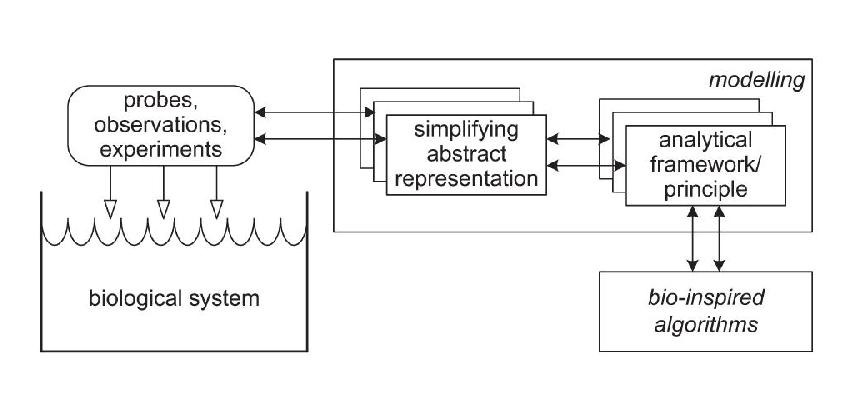
\includegraphics[scale=0.70]{Background/meth-conceptualframework}
	\caption{Depiction of the conceptual framework for devising Biological Inspired Algorithms, taken from \cite{Stepney2005}}
	\label{pic:meth-conceptualframework}
\end{figure}

%
% Immunology as Information Processing
%
\subsubsection{Immunology as Information Processing}
\label{subsec:iip}
Forrest and Hofmeyr summarised their AIS research efforts at the University of New Mexico and the Santa~Fe Institute as ``\emph{immunology as information processing}'' \cite{Forrest2001}. They define information as spatio-temporal patterns that can be abstracted and described independent of the biological system, and information processing as computation with these patterns. They proposed that such patterns are encoded in the proteins and other molecules of the immune system, and that they govern the behaviour of the biological system. They suggest that their information processing perspective can be contrasted with the conventional structural perspective of cellular interactions as mechanical devices. They consider a simple four-step procedure for the investigation of \emph{immunology as information processing}, transitioning from the biological system to a usable computational tool:

\begin{enumerate}
	\item Identify a specific mechanism that appears to be interesting computationally.
	\item Write a computer program that implements or models the mechanism.
	\item Study its properties through simulation and mathematical analysis.
	\item Demonstrate capabilities either by applying the model to a biological question of interest or by showing how it can be used profitably in a computer science setting.
\end{enumerate}

The procedure is similar to the outlined in the conceptual framework for Biologically Inspired Algorithms in that in addition to identifying biological mechanisms (input) and demonstrating a resultant algorithms (output), the procedure (1) highlights the need for abstraction involving modelling the identified mechanism, and (2) highlights the need to analyse the models and abstractions. The procedure of Forrest and Hofmeyr can be used to specialise Stepney, et~al. conceptual framework by clearly specifying the immunological information processing focus.

%
% Experimental Methodology
% Taken from: A Note on Research Methodology and Benchmarking Optimization Algorithms
% 
\subsection{Experimental Methodology}
\label{subsec:methodology:experimental}
% introduce optimization
Optimization is a generalized class of problem involving improvement of a structure under a cost function. It is a one of a few standard perspectives for the investigation and application for computational intelligence systems, specifically including clonal selection algorithms. As such, this section considers the state of optimization algorithm experimental methodology, the concerns of which are applicable to the investigation of computational intelligence algorithms in general.

% into optimization
When it comes to evaluating an optimisation algorithm, every researcher has their own thoughts on the way in which to proceed. Unfortunately, many empirical evaluations of optimisation algorithms are performed and reported without addressing basic experimental design considerations. Perhaps before an experimental methodology can be adopted, a researcher or practitioner may be paralysed by the perceived pessimism of the \emph{no free lunch} theorem that contends the futility of the benchmarking exercise. A pervasive problem in the field of Computational Intelligence algorithms is the lack of meaningful and consistent algorithm experimental and benchmarking methodology. This includes but is not limited to issues of the selection of problem instances, the selection of algorithm specifications, the algorithm configuration parameters, and interpretation of results. The intention of this section is to summarise the general concerns of experimental methodology, with a focus on benchmarking Computational Intelligence algorithms in the face of the `no free lunch' theorem.

%
% No Free Lunch
%
\subsubsection{No Free Lunch}
Wolpert and Macready's \emph{No Free Lunch Theorem} of search and optimisation has caused a lot of pessimism and misunderstanding, particularly in related to the evaluation and comparison of computational intelligence algorithms \cite{Wolpert1997, Wolpert1995}. In simplest terms, the theory indicates that when searching for an extremum of a cost function, \emph{all algorithms perform the same when averaged over all possible cost functions}. The implication is that the often perused general-purpose optimisation algorithm is theoretically impossible. The theory applies to stochastic and deterministic optimisation algorithms, and to algorithms that learn and adjust their search strategy over time. It is invariant to the performance measure used as well as the representation selected. Perhaps the catalyst for benchmarking cynicism is a comment accompanying the proof suggesting that: ``\ldots \emph{comparisons reporting the performance of a particular algorithm with a particular parameter setting on a few sample problems are of limited utility}'' \cite{Wolpert1997}.
% more
The theorem is an important contribution to computer science, although its implications are theoretical. The original paper was produced at a time when grandiose generalisations were being made as to algorithm, representation, or configuration superiority. The practical impact of the theory is to \emph{bound claims of applicability}. Wolpert and Macready encouraged effort be put into devising practical problem classes and the matching of suitable algorithms to problem classes. Further they compelled practitioners to exploit domain knowledge in optimisation algorithm application, now an axiom in the field. 

%
% Issues of Benchmarking Methodology
%
\subsubsection{Issues of Benchmarking Methodology}
Empirically comparing the performance of algorithms on problem instances is a staple for the fields of heuristics and Computational Intelligence, and the problems of effective comparison methodology have been discussed since the inception of these fields. Johnson suggested that the coding of an algorithm is the easy part of the process, that the difficult work is getting meaningful and publishable results \cite{Johnson2002}. He provides a very through list of questions to consider before \emph{racing} algorithms, as well as what he describes as his \emph{pet peeves} within the field of empirical algorithm research. Hooker (among others) condemns what he refers to as \emph{competitive testing} of heuristic algorithms, calling it \emph{fundamentally anti-intellectual} \cite{Hooker1995}. Hooker continues by strongly encouraging a rigorous methodology of what he refers to as \emph{scientific testing} where the aim is to investigate algorithmic behaviours. Barr, et~al. list a number of properties worthy of a heuristic method making a contribution, which can be paraphrased as; efficiency, efficacy, robustness, complexity, impact, generalisability and innovation \cite{Barr1995}. Barr, Golden et~al. specify a loose experimental set-up methodology with the following intuitive steps; 1) define the goals of the experiment, 2) select measure of performance and factors to explore, 3) design and execute the experiment, 4) Analyse the data and draw conclusions, and finally 5) report the experimental results. They then suggest eight guidelines for reporting results, in summary they are; reproducibility, specify all influential factors (for example code and computing environment), be precise regarding measures, specify parameters, use statistical experimental design, compare with other methods, reduce variability of results, ensure results are comprehensive. 

Peer, et~al. summarise the problems of algorithm benchmarking (with a bias toward Particle Swarm Optimisation) to the following points; duplication of effort, insufficient testing, failure to test against state-of-the-art, poor choice of parameters, conflicting results, and invalid statistical inference \cite{Peer2003}. Eiben and Jelasity site four problems with the state of benchmarking evolutionary algorithms; (1) test instances are chosen ad~hoc from the literature, (2) results are provided without regard to research objectives, (3) scope of generalised performance is generally too broad, and (4) results are hard to reproduce \cite{Eiben2002}. 
% overview
The general problems with benchmarking methodology may be distilled into the following sub-problems:

\begin{itemize}
	\item \emph{Parameter Selection}: Computational Intelligence algorithms are typically parameterised, although the mapping of parameter values to predictable effects on problem domains is generally poorly understood. This is because typically unknown and non-linear dependencies commonly exist between the variables resulting in the algorithm being consider a complex system. Francois and Lavergne discuss the deficiencies of the traditional \emph{trial-and-error} and the \emph{experienced-practitioner} approaches to parameter tuning, further suggesting that seeking general rules for parameterisation will lead to optimisation algorithms that offer neither convergent or efficient behaviours \cite{Francois2001}. There are many solutions not limited to the following: consulting the literature although often ignored \cite{Eiben2002}), generalise from large numbers of experiments \cite{Schaffer1989}, self-adaptive parameters, meta-algorithms for searching for good parameters values, and statistical sensitivity analysis over parameter ranges \cite{Chan1997, Birattari2002}. 
	
	\item \emph{Problem Selection}: Problem instances should be selected to demonstrate specific behaviours of the systems under study. Typically benchmarks are performed on ad~hoc lists of standard benchmark instances, that although offering the benefit of comparability, typically devolve into racing contest. Eiben and Jelasity support the division of problem instances into categories and encourage the evaluation of optimisation algorithm over a large number of test instances \cite{Eiben2002}. In their paper on understanding the interactions of Genetic Algorithm parameters Deb and Agrawal propose four structural properties of problems for testing genetic algorithms; multi-modality, deception, isolation, and collateral noise \cite{Deb1999}. Yao, et~al.  divide their large test dataset into the categories of uni-modal, multi-modal with many local optima, and multi-modal with few local optima \cite{Yao1999}. Whitley, et~al.  provide a detailed study on the problems of selecting test instances for genetic algorithms, and suggest that difficult problem instances should be non-linear, non-separable, and non-symmetric \cite{Whitley1996}.
	
	\item \emph{Measure Selection}: There are many ways to measure the performance of an algorithm for a problem instance, although the most common involves measures of \emph{efficacy} (problem specific costs) and \emph{efficiency} (computation space and/or time). Most Biologically Inspired Algorithms have a stochastic element, typically in their random starting position(s) and in the probabilistic decisions made during sampling of the domain. Therefore, the measuring of performance must be repeated a number of times to account for the stochastic variance\footnote{Typically $\geq30$ according to the central limit theorem such that the underlying distribution can be meaningfully summarised.}, which also could be a measure of comparison between algorithms. The most critical concern in the selection of measures is that of standardisation for the purposes of comparison \cite{Birattari2005a, Barr1995}.	
	
	\item \emph{Statistical Significance}: The scientific knowledge of Computational Intelligence is predominantly accrued as empirical observations and conclusions. Therefore, there is a need for methods that permit interpretation and conclusions to be drawn beyond the standard reporting of results. Statistical hypothesis testing and related methods provides such tools, although unfortunately are rarely employed. Peer, et~al. \cite{Peer2003} and Birattari and Dorigo \cite{Birattari2005} provide a basic introduction (suitable for an algorithm-practitioner) into the appropriateness of various statistical tests for algorithm comparisons. Parametric statistical methods are used for interval and ratio data (like a real-valued performance measure), and non-parametric methods are used for ordinal, categorical and rank-based data. Interval data is typically converted to ordinal data when salient constraints of desired parametric tests (such as assumed normality of distribution) are broken such that the less powerful non-parametric tests can be used. The use of non-parametric statistical tests maybe preferred as some authors (for example \cite{Chiarandini2005}) claim the distribution of cost values are very asymmetric and/or not Normal.
\end{itemize}

%
% Integrated Methodology
% Taken from 'Small Models': A Methodology for Designing and Investigating Adaptive Systems
%
% Omitted the genetic algorithm Section~(ga, innovation)
% 
\subsection{Designing and Investigating Adaptive Systems}
\label{subsec:smallmodels}
Complex and adaptive systems are difficult to design and investigate, therefore the need for a coherent and proven methodology for such activities is paramount. Inspired by an interpretation of the achievements of the Wright brothers in achieving the first powered flight, this section provides a summary of a methodology for investigating and designing \emph{conceptual machines} proposed by David Goldberg \cite{Goldberg2002}. 

For the purposes of clarity, a \emph{model} is a conceptualisation that provides a description of a system that accounts for its properties and may be used to study the characteristics of the system. For the remainder of this thesis, conceptual models are instantiated as \emph{algorithms} for the purposes of computational implementation, simulation, and study. The algorithms provide procedures for problem-solving when the behaviour of the instantiated model suitably match the characteristics of a problem.

%
% Engineers and Mathematicians
%
\subsubsection{Engineers and Mathematicians}
Goldberg describes the airplane and other products of engineering as \emph{material machines}, and distinguishes them from the engineering of genetic algorithms and other adaptive systems as \emph{conceptual machines}. He argues the methodological distinction between the two is counter-productive and harmful from the perspective of conceptual machines, specifically that the methodology of the material is equally applicable to that of the conceptual \cite{Goldberg1999a}. The obsession of mathematical rigour in computer science, although extremely valuable, is not effective in the investigation of adaptive systems given their complexity. Goldberg sights the airplane as an example where the engineering invention is used and trusted without a formal proof that the invention works (that an airplane can fly\footnote{Goldberg is quick to point out that sets of equations do exist for various aspects of flight, although no integrated mathematical proof for airplane flight exists.}). This defence leads to what Goldberg refers to the \emph{economy of design} which is demonstrated with a trade-off that distinguishes `model description' (mathematician-scientists) that is concerned with model fidelity, and model prescription (engineer-inventor) that is concerned with a working product. In descriptive modelling \emph{the model is the thing} (of interest) whereas in `prescriptive modelling', \emph{the object is the thing} (of interest). In the latter, the model (and thus its utility) serves the object, in the former model accuracy may be of primary concern. This economy of modelling provides a perspective that distinguishes the needs of the prescriptive and descriptive fields of investigation. 

The mathematician-scientist is interested in increasing model accuracy at the expense of the speed (slow), where as the engineer may require a marginally predictive (inaccurate) model relatively quickly. This trade-off between high-cost high-accuracy models and low-cost low-fidelity models is what may be referred to as the \emph{modelling spectrum} that assists in selecting an appropriate level of modelling. Goldberg proposes that the field of genetic algorithms expend too much effort at either ends of this spectrum. There is much work where there is an obsession with blind-prototyping many different tweaks in the hope of striking it lucky with the \emph{right} mechanism, operator, or parameter. Alternatively, there is also an obsession with detailed mathematical models such as full-blown differential equations and Markov chains. The middle ground of the spectrum, what Goldberg refers to as \emph{little models} is a valuable economic modelling consideration for the investigation of conceptual machines to \emph{do good science through good engineering}. 

%
% Methodology
%
\subsubsection{Methodology}
The methodology has been referred to as post-modern systems engineering and is referred to by Goldberg as a methodology of innovation \cite{Goldberg2004}. The core principles of the process are as follows: 

\begin{enumerate}
	\item \emph{Decomposition}: Decompose the large problem approximately and intuitively, breaking into quasi-separate sub-problems.
	\item \emph{Modelling}: Investigate each sub problem separately (or as separate as possible) using empirical testing coupled with adequately predictive, low-cost models.
	\item \emph{Integration}: Assemble the sub-solutions and test the overall invention, paying attention to unforeseen interactions between the sub-problems.
\end{enumerate}

%
% Decomposition
%
\paragraph{Decomposition} Problem decomposition and decomposition design is an axiom of reductionism and is at the very heart of problem solving in computer science. Therefore, it is not worth dwelling on the topic other than to comment as to its meaning within the context of adaptive systems. One may consider the base or medium on which the system is performing its computation mechanisms, the so-called building blocks of information processing. A structural decomposition may involve the architecture and data structures of the system. Additionally, one may also consider a functional breakdown of mechanisms such as the operators applied at each discrete step of an algorithmic process or mechanisms. The reductions achieved provide the basis of investigation and modelling.

%
% Small Models
%
\paragraph{Small Models} Given the principle of the economy of modelling presented as a spectrum, one may extend the description of each of the five presented model types. \emph{Small Models} refers to the middle of the spectrum, specifically to the application of dimensional and facet-wise models. These are mid-range quantitative models that make accurate prediction over a limited range of states at moderate cost. Once derived, this class of models generally requires a small amount of formal manipulation and large amounts of data for calibration and verification. The following summarises the modelling spectrum:

\begin{itemize}
	\item \emph{Unarticulated Wisdom}: (low-cost, high-error) Intuition, what is used when there is nothing else.
	\item \emph{Articulated Qualitative Models}: Descriptions of mechanisms, graphical representations of processes and/or relationships, empirical observation or statistical data collection and analysis.
	\item \emph{Dimensional Models}: Investigate dimensionless parameters of the system.
	\item \emph{Facet-wise Models}: Investigation of a decomposition element of a model in relative isolation.
	\item \emph{Equations of Motion}: (high-cost, low-error) Differential equations and Markov chains.
\end{itemize}

Facet-wise models are an exercise in simple mathematics that may be used to investigate a decomposition element of a model in relative isolation. They are based on the idea of \emph{bracketing high-order phenomena} by simplifying or making assumptions about the state of the system. An example used by Goldberg from fluid mechanics is a series of equations that simplify the model by assuming that a fluid or gas has no viscosity, which matches no known substance. A common criticism of this modelling approach is ``\emph{system X doesn't work like that, the model is unrealistic}''. The source of such concerns with adaptive systems is that their interactions are typically high-dimensional and non-linear. Goldberg's response is that for a given poorly understood area of research, any useful model is better than no model. Dimensional analysis or the so-called dimensional reasoning and scaling laws are another common conceptual tool in engineering and the sciences. Such models may be used to investigate dimensionless parameters of the system, which may be considered the formalisation of the systemic behaviours.

%
% Integration
%
\paragraph{Integration} Integration is a unification process of combining the findings of various models together to form a \emph{patch-quilt} coherent theory of the system. Integration obviously is not limited to holistic unification, one may address specific hypothesis regarding the system resulting in conclusions about existing systems, and design decisions pertaining to the next generation of systems.

%
% Application
%
\paragraph{Application} In addition to elucidating the methodology, Goldberg specifies a series of five useful heuristics for the application of the methodology as follows (taken from \cite{Goldberg1999a}, page 8):

\begin{enumerate}
	\item \emph{Keep the goal of a working conceptual machine in mind}. Experiments commonly get side tracked by experimental design and statistical verification; theoreticians get side tracked with notions of mathematical rigour and model fidelity.
	\item \emph{Decompose the design ruthlessly}. One cannot address the analytical analysis of a system like a genetic algorithm in one big `gulp'.
	\item \emph{Use facet-wise models with almost reckless abandon}. One should build easy models that can be solved by bracketing everything that gets in the way.
	\item \emph{Integrate facet-wise models using dimensional arguments}. One can combine many small models together in a patch-quilt manner and defend the results of such models using dimensional analysis.
	\item \emph{Build high-order models when small models become inadequate}. Add complexity to models as complexity is needed (economy of modelling).
\end{enumerate}

%
% Summary
% Provides an overview of the chapter and its structure, and a description of what is intended to be achieved by providing this documentation. A description of why and how this chapter follows on from the previous chapter
%
\section{Chapter Summary}
\label{sec:background:summary}
% broad position
This Chapter positioned the investigation broadly in the field of Biologically Inspired Computational Intelligence, a sub-field of Artificial Intelligence, and specifically in the field of Artificial Immune Systems. 
% motivation - clonal selection
Clonal Selection was highlighted as an adaptive paradigm in the field of Artificial Immune Systems that underlies much of the general field.
% motivation - distributed
Distributed Artificial Immune Systems including distributed Clonal Selection Algorithms is an over promised and under delivered, although potentially beneficial field of study. An effective realisation of distributed clonal selection algorithms is expected to facilitate the broader application of such approaches to classes of problem that may benefit from parallel and cooperative problem solving strategies, such as problems with functional or information availability decompositions.
% motivation - using biology
Turning back to the structure and function of the immune system to develop new AIS approaches including distributed approaches is currently an advocated approach in the field given the apparent impasse experienced in the progress of such approaches. 
% methodology
A systematic framework was adopted for the development of new immunologically inspired approaches, with careful empirical investigation, and awareness of the economy of models and need for the re-integration of findings.
% next
This chapter both positioned and motivated the research hypothesis outlined in Chapter \ref{chap:introduction}, and defined the systematic methodology adopted for the development and investigation of adaptive and distributed clonal selection algorithms throughout the remainder of the dissertation. Toward this end, Chapter \ref{chap:cs} provides an in depth investigation into the clonal selection paradigm, both reviewing and elaborating the cellular perspective of such approaches which is later pursued in Chapter \ref{chap:cells}, and outlining the agenda for realising distributed approaches in Chapters \ref{chap:tissues} and \ref{chap:hosts}.

% EOF